\section{Results (\textit{Jacob Salomonsen})}



\subsection{Running time}
After running the test described in \autoref{sec:testing} on both the CPU- and the GPU-version, we got the following results. \autoref{results} shows the resultant graphs by plotting the size of the simulated field against the the average column of \autoref{resultcpu} and \autoref{resultgpu}.

\insfig{./images/result.png}{1.0\textwidth}{results}{results}

The graphs on \autoref{results} shows a clear sign that the GPU-based version is faster than the CPU-based version, but that the implementations also exhibit the same time complexity. The graphs have the same shape and are reminiscent of a quadratic functions. Although this can be observed, is is beyond the scope of this report to verify it.



\subsection{Other characteristics}
As a secondary result, the result of simulating the lid driven cavity can be compared with a reference from another implementation, as to see if the implementation performs in the way one would expect. In \autoref{lidimages}, the reference images is \autoref{lidref}, taken from \cite{lidref}. Although they are not exactly the same our implementation exhibits the same pattern as in the reference solution.


\begin{figure}[H]
\centering
\subfigure[Lid driven cavity flow calculated by PyCUDA]{
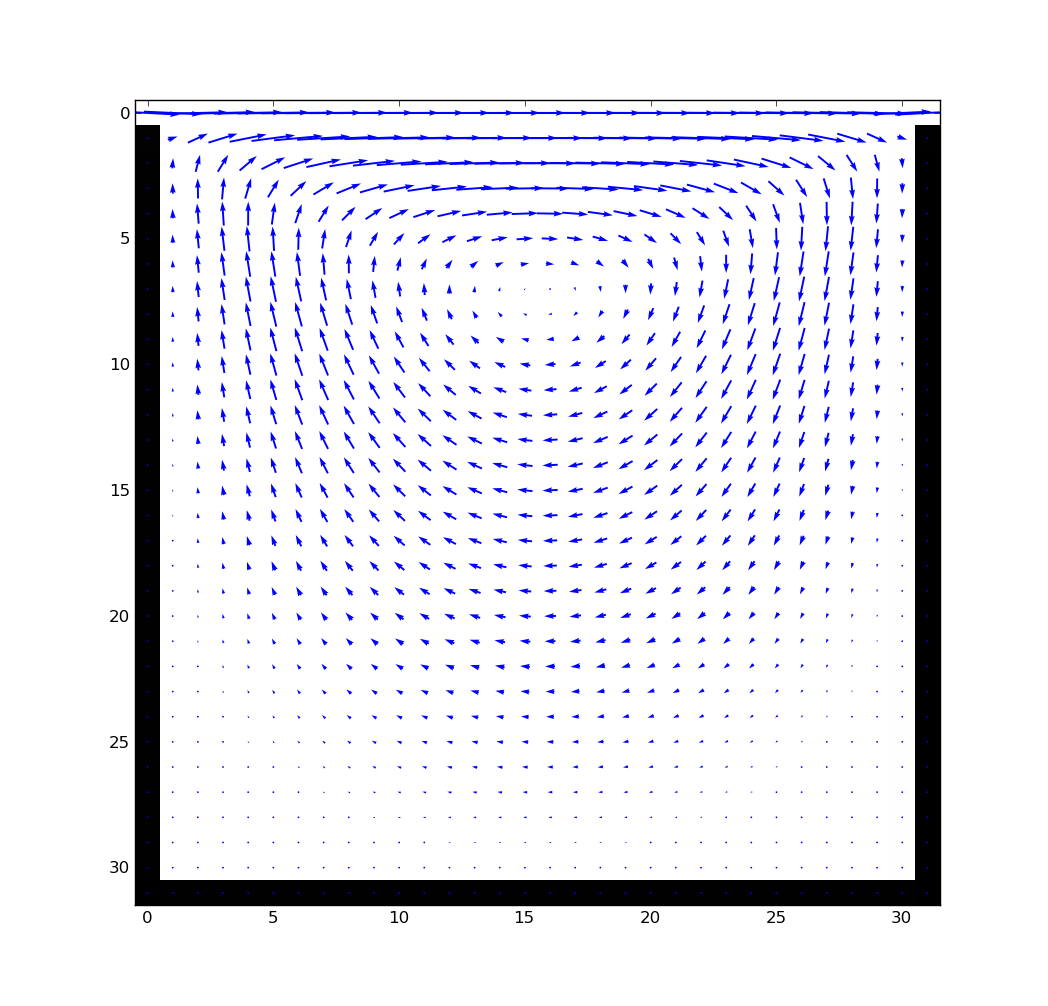
\includegraphics[width=0.47\textwidth]{./images/cuda_lid_32_32_900.png}
\label{lid}
}
\hspace{1pt}
\subfigure[The same simulation as in \autoref{lid}, but with color gradient]{
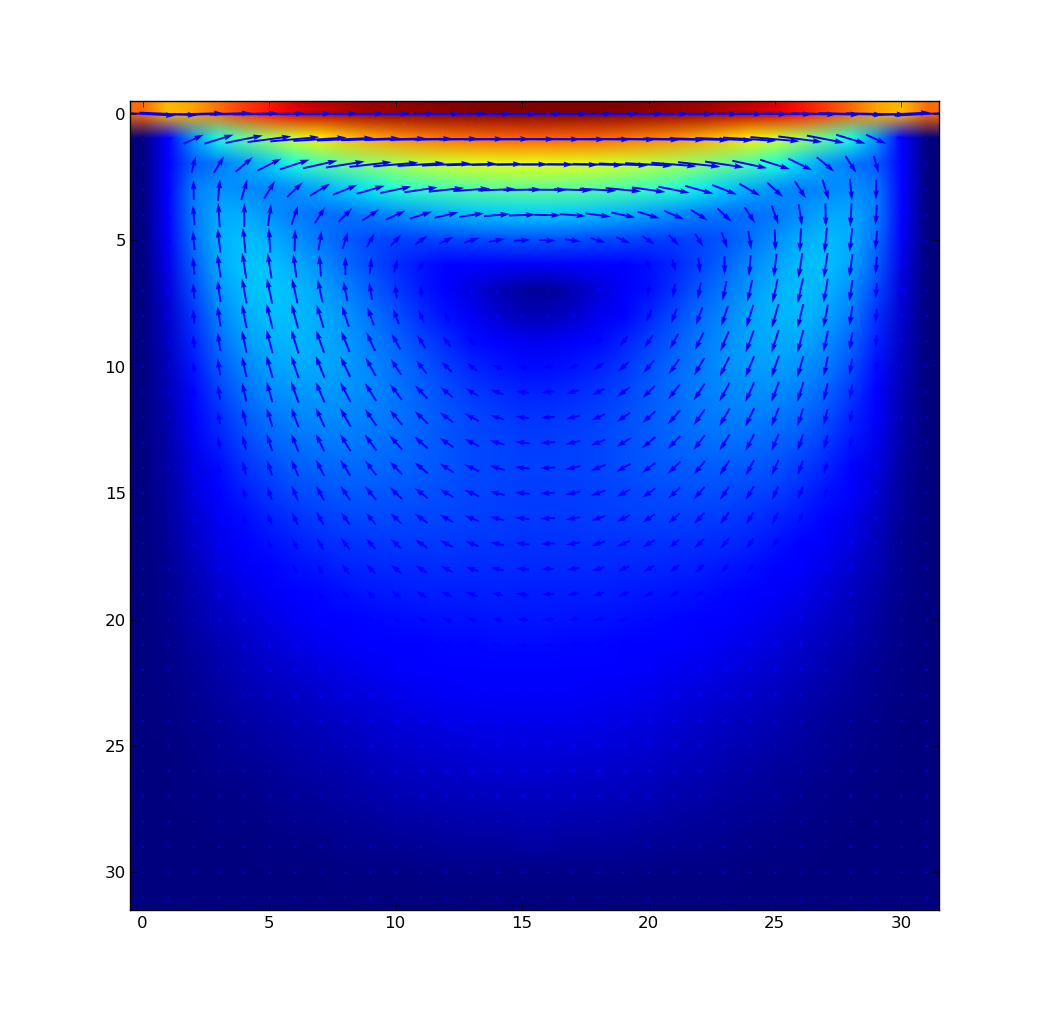
\includegraphics[width=0.47\textwidth]{./images/cuda_lid_32_32_900_color.png}
\label{lidcolor}
}

\subfigure[A lid driven cavity consisting of 256x256 nodes after 2700 iterations]{
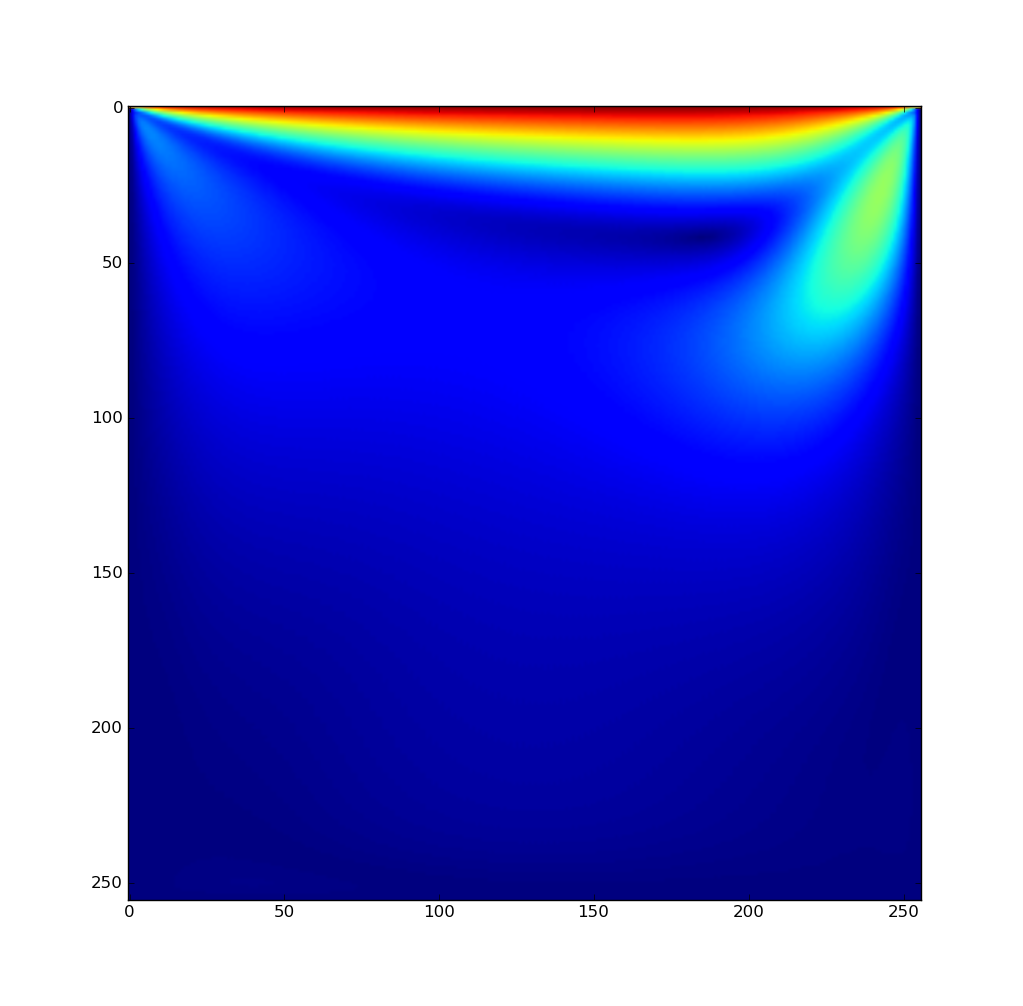
\includegraphics[width=0.47\textwidth]{./images/cuda_lid_256_256_2700.png}
\label{lidhighit}
}
\hspace{1pt}
\subfigure[Reference lid driven cavity simulation taken from \cite{lidref}]{
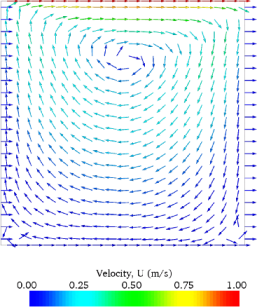
\includegraphics[width=0.35\textwidth]{./images/lidref.png}
\label{lidref}
}
\caption{Lid driven cavity simulation}
\label{lidimages}
\end{figure}


